% --- Page Style ---
\pagestyle{fancy}
\fancyhf{}
\lhead{SAT}
% \rhead{Exam ID: \underline{\hspace{2cm}}}
\lfoot{Practice Exam}
\rfoot{Page \thepage}
\renewcommand{\headrulewidth}{0.4pt}
\renewcommand{\footrulewidth}{0.4pt}

% --- Header spanning both columns ---
\twocolumn[
  \begin{center}
    {\huge \textbf{SAT Practice Exam}} \\
    \vspace{0.2cm}
    {\large \textbf{No Calculator \& Calculator-Allowed Sections}} \\
    \vspace{0.4cm}
    \begin{tabular}{|l|l|}
      \hline
      \textbf{Student Name:} & \hspace{6cm} \\ \hline
      \textbf{Date:} & \hspace{6cm} \\ \hline
    \end{tabular}
  \end{center}
  \vspace{0.6cm}
  \textbf{Instructions:} Answer each question. For multiple-choice questions, choose the best answer from (A)--(D). For grid-in questions, write your answer in the box. No calculator is allowed for Part I; a calculator is allowed for Part II.
  \vspace{0.8cm}
]

% --- Questions ---

\section*{Part I: No Calculator SAT Math Questions}

\begin{enumerate}[leftmargin=*, label=\textbf{\arabic*.}]

  \item
  \[
  C = \frac{5}{9}(F - 32)
  \]
  The equation above shows how temperature $F$, measured in degrees Fahrenheit, relates to a temperature $C$, measured in degrees Celsius. Based on the equation, which of the following must be true?

  \textbf{I.} A temperature increase of 1 degree Fahrenheit is equivalent to a temperature increase of $\frac{5}{9}$ degree Celsius.

  \textbf{II.} A temperature increase of 1 degree Celsius is equivalent to a temperature increase of 1.8 degrees Fahrenheit.

  \textbf{III.} A temperature increase of $\frac{5}{9}$ degree Fahrenheit is equivalent to a temperature increase of 1 degree Celsius.

  \begin{tasks}(2)
    \task I only
    \task II only
    \task III only
    \task I and II only
  \end{tasks}
  \vspace{1cm}



  \item The equation $\displaystyle \frac{24x^2 + 25x - 47}{ax - 2} = -8x - 3 - \frac{53}{ax - 2}$ is true for all values of $x \neq \frac{2}{a}$, where $a$ is a constant. What is the value of $a$?

  \begin{tasks}(2)
    \task $-16$
    \task $-3$
    \task $3$
    \task $16$
  \end{tasks}
  \vspace{4cm}

  \item If $3x - y = 12$, what is the value of $\displaystyle \frac{8^x}{2^y}$?

  \begin{tasks}(1)
    \task $2^{12}$
    \task $4^4$
    \task $8^2$
    \task The value cannot be determined from the information given.
  \end{tasks}
  \vspace{4cm}

  \item Points $A$ and $B$ lie on a circle with radius 1, and arc $\stackrel{\frown}{AB}$ has length $\frac{\pi}{3}$. What fraction of the circumference of the circle is the length of arc $\stackrel{\frown}{AB}$?
  \vspace{4cm}

  \newpage
  \item The expression $\displaystyle \frac{8 - i}{3 - 2i}$ is rewritten in the form $a + bi$, where $a$ and $b$ are real numbers. What is the value of $a$? (Note: $i = \sqrt{-1}$.)
  \vspace{4cm}

  \item In triangle $ABC$, the measure of $\angle B$ is $90^\circ$, $BC = 16$, and $AC = 20$. Triangle $DEF$ is similar to triangle $ABC$, with vertices $D$, $E$, and $F$ corresponding to $A$, $B$, and $C$ respectively, and each side of triangle $DEF$ is $\frac{1}{3}$ the length of the corresponding side of triangle $ABC$. What is the value of $\sin F$?
  \vspace{4cm}

\end{enumerate}


\newpage

\section*{Part II: Calculator-Allowed SAT Math Questions}

\begin{enumerate}[leftmargin=*, label=\textbf{\arabic*.}, resume]

  \item The incomplete table below summarizes the number of left-handed and right-handed students by gender for the eighth grade students at Keisel Middle School.
  \begin{center}
  \begin{tabular}{|l|c|c|}
    \hline
    & \textbf{Left-handed} & \textbf{Right-handed} \\ \hline
    \textbf{Male}   & \hspace{1.2cm} & \hspace{1.2cm} \\ \hline
    \textbf{Female} & \hspace{1.2cm} & \hspace{1.2cm} \\ \hline
    \textbf{Total} & 18 & 122 \\ \hline
  \end{tabular}
  \end{center} There are 5 times as many right-handed female students as left-handed female students, and 9 times as many right-handed male students as left-handed male students. If there are 18 left-handed students and 122 right-handed students in total, which of the following is closest to the probability that a right-handed student selected at random is female? (Assume that no eighth-grade student is both right-handed and left-handed.)

  \begin{tasks}(2)
    \task 0.410
    \task 0.357
    \task 0.333
    \task 0.250
  \end{tasks}
  \vspace{4cm}


  \newpage

  \textbf{For questions 8 and 9, use the following information.} 
  
  If shoppers enter a store at an average rate of $r$ shoppers per minute and each stays an average of $T$ minutes, the average number of shoppers in the store, $N$, at any one time is $N = rT$ (Little's law). The owner of the Good Deals Store estimates that during business hours, an average of 3 shoppers per minute enter the store and each stays an average of 15 minutes, so there are about 45 shoppers in the store at any time.

  \item Little's law can be applied to any part of the store. The store owner determines that during business hours, approximately 84 shoppers per hour make a purchase and each spends an average of 5 minutes in the checkout line. At any time during business hours, about how many shoppers, on average, are waiting in the checkout line to make a purchase at the Good Deals Store?
  \vspace{4cm}

  \item The owner opens a new store across town. For the new store, an average of 90 shoppers per hour enter and each stays an average of 12 minutes. The average number of shoppers in the new store at any time is what percent less than the average number in the original store? (Ignore the percent symbol when entering your answer; e.g., if the answer is 42.1\%, enter 42.1.)
  \vspace{4cm}



  \newpage

  \item In the $xy$-plane, the point $(p, r)$ lies on the line $y = x + b$, and the point $(2p, 5r)$ lies on the line $y = 2x + b$, where $b$ is a constant. If $p \neq 0$, what is the value of $\frac{r}{p}$?

  \begin{tasks}(3)
    \task $\frac{2}{5}$
    \task $\frac{3}{4}$
    \task $\frac{4}{3}$
  \end{tasks}
  \vspace{4cm}

  \item A grain silo is built from two right circular cones and a right circular cylinder with internal measurements represented by the figure below. Of the following, which is closest to the volume of the grain silo, in cubic feet?
  \begin{center}
  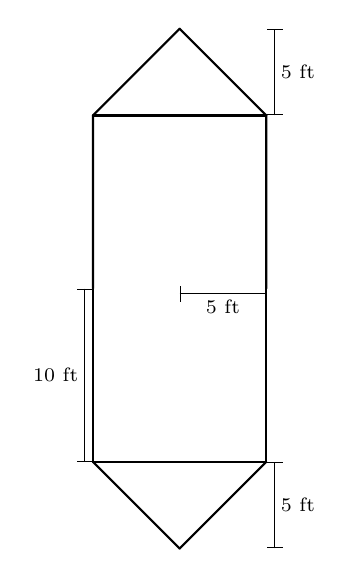
\begin{tikzpicture}[x=0.22cm, y=0.22cm, line cap=round, line join=round]
    % Silo: radius 5 ft, cylinder height 10 ft, each cone height 5 ft.
    % Drawing scale: 1 unit = 1 ft so proportions are exact.
    \def\r{5}
    \def\Hcyl{10}
    \def\Hcone{5}
    % Top cone
    \draw[thick] (0,\Hcyl+\Hcone) -- (-\r,\Hcyl) -- (-\r,0);
    \draw[thick] (0,\Hcyl+\Hcone) -- (\r,\Hcyl) -- (\r,0);
    \draw[thick] (-\r,\Hcyl) -- (\r,\Hcyl);
    % Cylinder
    \draw[thick] (-\r,0) -- (-\r,-\Hcyl);
    \draw[thick] (\r,0) -- (\r,-\Hcyl);
    \draw[thick] (-\r,-\Hcyl) -- (\r,-\Hcyl);
    % Bottom cone
    \draw[thick] (-\r,-\Hcyl) -- (0,-\Hcyl-\Hcone);
    \draw[thick] (\r,-\Hcyl) -- (0,-\Hcyl-\Hcone);
    % Dimension labels: radius 5 ft, cylinder body full height 10 ft (left), cones 5 ft (right)
    \draw[|-|] (-\r-0.5,0) -- (-\r-0.5,-\Hcyl) node[midway,left,inner sep=2pt] {\scriptsize 10 ft};
    \draw[|-|] (0,-0.3) -- (\r,-0.3) node[midway,below,inner sep=2pt] {\scriptsize 5 ft};
    \draw[|-|] (\r+0.5,\Hcyl) -- (\r+0.5,\Hcyl+\Hcone) node[midway,right,inner sep=2pt] {\scriptsize 5 ft};
    \draw[|-|] (\r+0.5,-\Hcyl-\Hcone) -- (\r+0.5,-\Hcyl) node[midway,right,inner sep=2pt] {\scriptsize 5 ft};
  \end{tikzpicture}
  \end{center}

  \begin{tasks}(2)
    \task 261.8
    \task 785.4
    \task 916.3
    \task 1047.2
  \end{tasks}
  \vspace{4cm}

  \newpage
  \item If $x$ is the average (arithmetic mean) of $m$ and 9, $y$ is the average of $2m$ and 15, and $z$ is the average of $3m$ and 18, what is the average of $x$, $y$, and $z$ in terms of $m$?

  \begin{tasks}(2)
    \task $m + 6$
    \task $m + 7$
    \task $2m + 14$
    \task $3m + 21$
  \end{tasks}
  \vspace{4cm}

  \item The function $f(x) = x^3 - x^2 - x - \frac{11}{4}$ is graphed in the $xy$-plane below. If $k$ is a constant such that the equation $f(x) = k$ has three real solutions, which of the following could be the value of $k$?
  \begin{center}
  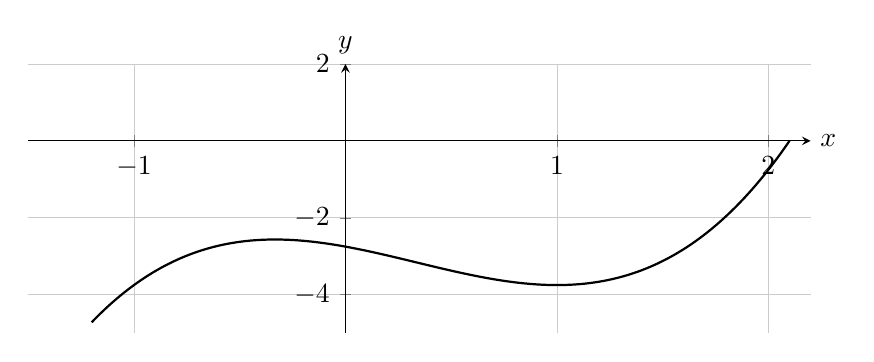
\begin{tikzpicture}[baseline=(current bounding box.center)]
    \begin{axis}[
      width=0.95\linewidth,
      height=5cm,
      axis lines=middle,
      xlabel={$x$},
      ylabel={$y$},
      xlabel style={at=(ticklabel* cs:1), anchor=west},
      ylabel style={at=(ticklabel* cs:1), anchor=south},
      xmin=-1.5, xmax=2.2,
      ymin=-5, ymax=2,
      xtick={-1,0,1,2},
      ytick={-4,-2,0,2},
      grid=both,
      grid style={line width=.3pt, draw=gray!40},
      samples=80,
      smooth,
    ]
      \addplot[thick, domain=-1.2:2.1] {x^3 - x^2 - x - 11/4};
    \end{axis}
  \end{tikzpicture}
  \end{center}
  \vspace{4cm}


  \newpage
  \item The dynamic pressure $q$ generated by a fluid moving with velocity $v$ is given by
  \[
  q = \frac{1}{2} n v^2,
  \]
  where $n$ is the constant density of the fluid. An aeronautical engineer uses the formula to find the dynamic pressure of a fluid moving with velocity $v$ and with velocity $1.5v$. What is the ratio of the dynamic pressure of the faster fluid to the dynamic pressure of the slower fluid?
  \vspace{4cm}

  \item For a polynomial $p(x)$, the value of $p(3)$ is $-2$. Which of the following must be true about $p(x)$?

  \begin{tasks}(1)
    \task $x - 5$ is a factor of $p(x)$.
    \task $x - 2$ is a factor of $p(x)$.
    \task $x + 2$ is a factor of $p(x)$.
    \task The remainder when $p(x)$ is divided by $x - 3$ is $-2$.
  \end{tasks}
  \vspace{4cm}

\end{enumerate}
